\subsection{Package sequenziatore::server::presenter}
\begin{figure}[H] \centering 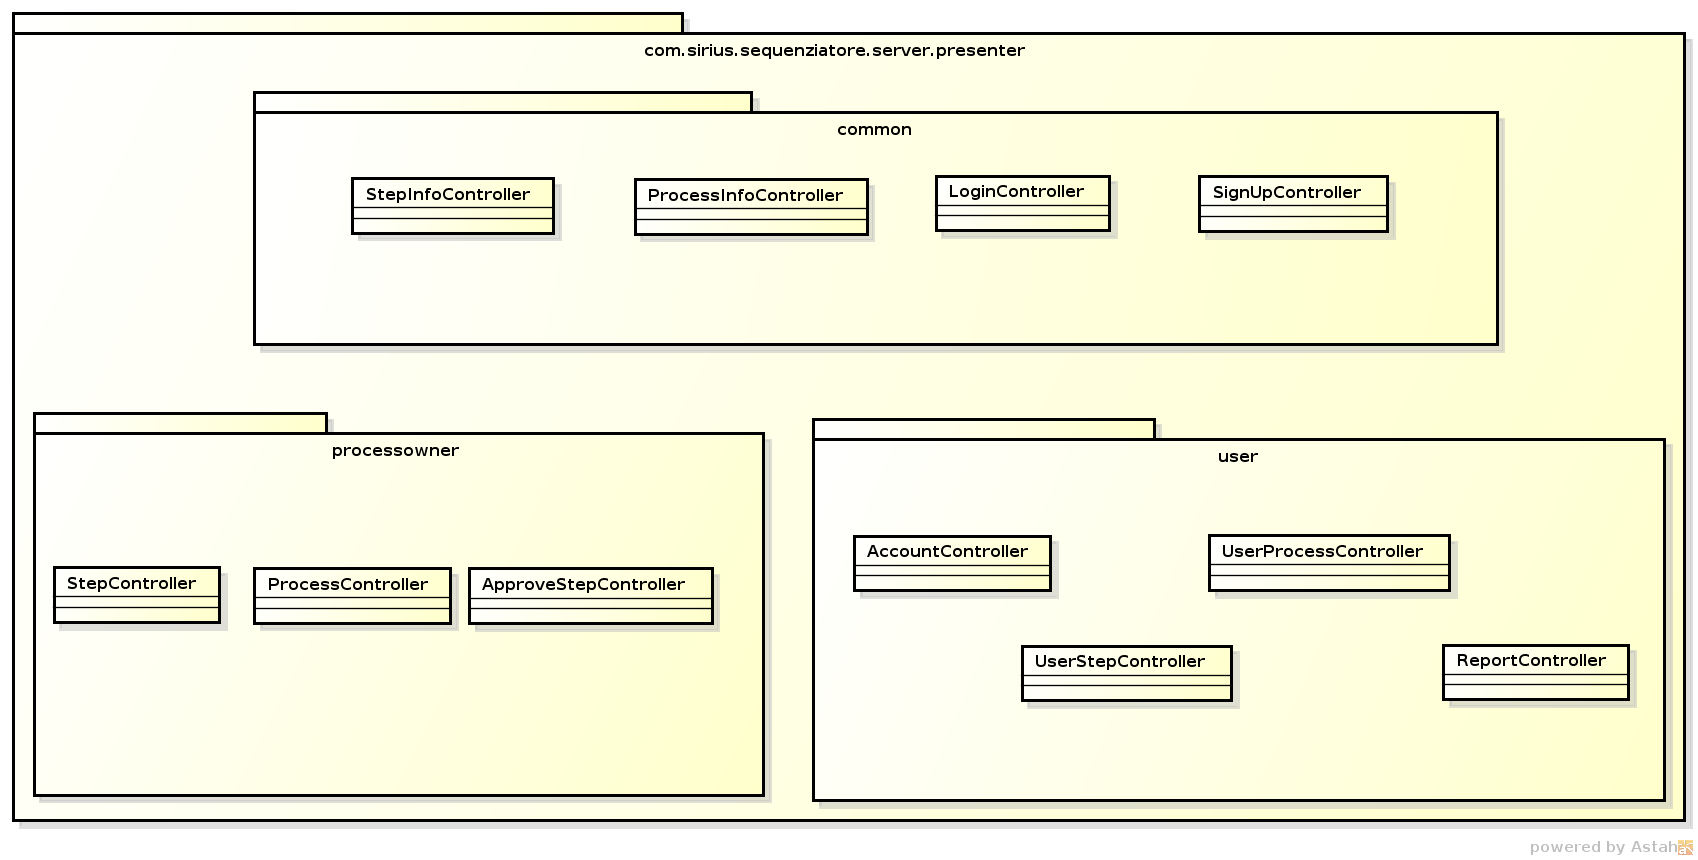
\includegraphics[width=%
\textwidth]
{./pack/ClassiServerSoloPresenter.png} \caption{Diagramma presenter server}
\end{figure}
\paragraph{PresenterFacade}
	\begin{itemize}
		\item \textbf{Nome:} \texttt{PresenterFacade}
		\item \textbf{Tipo:} Abstract;
		\item \textbf{Package:} sequenziatore::server::presenter
		\item \textbf{Descrizione:} Classe astratta che ha il ruolo di decidere a che pacchetto inoltrare le richieste;
		\item \textbf{Relazione con altre componenti:} la classe richiama metodi delle classi:
		\begin{itemize}
			\item sequenziatore::server::presenter::iprocessowner::ProcessOwnerFacade;
			\item sequenziatore::server::presenter::iprocessowner::UserFacade.
		\end{itemize}
	\end{itemize}
%00000000000000000000000000000000000000000000000000000000000000000000000000000000000000000000000000000%
\subsubsection{Package sequenziatore::server::presenter::iclientcommunication}
\paragraph{ICommunication}
	\begin{itemize}
		\item \textbf{Nome:} \texttt{ICommunication};
		\item \textbf{Tipo:} Interface;
		\item \textbf{Package:} sequenziatore::server::presenter::iclientcommunication
		\item \textbf{Descrizione:} interfaccia che gestisce le comunicazioni con il \textit{presenter} lato \textit{client};
	\end{itemize}
%----------------------------------------------------------------------------------------------%
\paragraph{IDataFormatter}
	\begin{itemize}
		\item \textbf{Nome:} IDataFormatter;
		\item \textbf{Tipo:} Interface;
		\item \textbf{Package:} sequenziatore::server::presenter::iclientcommunication
		\item \textbf{Descrizione:} interfaccia che gestisce le comunicazioni con il presenter lato \textit{client} tramite richieste http;
	\end{itemize}
%0000000000000000000000000000000000000000000000000000000000000000000000000000000000000000000000000%
\subsubsection{Package sequenziatore::server::presenter::clientcommunication}
\paragraph{HttpCommunication}
	\begin{itemize}
		\item \textbf{Nome:} \texttt{HttpCommunication};
		\item \textbf{Tipo:} Class;
		\item \textbf{Package:} sequenziatore::server::presenter::clientcommunication
		\item \textbf{Descrizione:} classe responsabile della gestione delle comunicazioni con il presenter lato \textit{client} tramite richieste http;
		\item \textbf{Relazione con altre componenti:} la classe implementa l' interfaccia :\texttt{sequenziatore::server::presenter::iclientcommunication::ICommunication} e richiama metodi delle classi:
		\begin{itemize}
			\item sequenziatore::server::presenter::PresenterFacade.
		\end{itemize}
	\end{itemize}
%----------------------------------------------------------------------------------------------%
\paragraph{WebsocketCommunication}
	\begin{itemize}
		\item \textbf{Nome:} WebsocketCommunication;
		\item \textbf{Tipo:} Class;
		\item \textbf{Package:} sequenziatore::server::presenter::clientcommunication
		\item \textbf{Descrizione:} classe responsabile della gestione delle comunicazioni con il presenter lato \textit{client} tramite WebSocket;
		\item \textbf{Relazione con altre componenti:} la classe implementa l' interfaccia :\texttt{sequenziatore::server::presenter::iclientcommunication::ICommunication} e richiama metodi delle classi:
		\begin{itemize}
			\item sequenziatore::server::presenter::PresenterFacade.
		\end{itemize}
	\end{itemize}
%----------------------------------------------------------------------------------------------%
\paragraph{JSONFortmatter}
	\begin{itemize}
		\item \textbf{Nome:} JSONFormatter;
		\item \textbf{Package:} \texttt{sequenziatore::server::presenter::clientcommunication}
		\item \textbf{Descrizione:} classe responsabile del parsing dell'oggetto JSON;
		\item \textbf{Relazione con altre componenti:} la classe implementa l' interfaccia :\texttt{sequenziatore::server::presenter::iclientcommunication::IDataFormatter}
	\end{itemize}